\documentclass{article}
\usepackage[utf8]{inputenc}
\usepackage[english]{babel}
\usepackage{amsmath}
\usepackage{mathtools}
\usepackage{algorithmicx}
\usepackage{algorithm}
\usepackage{algpseudocode}
\makeatletter
\renewcommand{\ALG@name}{Pseudocode}
\makeatother

\usepackage{rotating}
\usepackage{hyperref}
\usepackage{todonotes}

\title{RandomMatrixChapter}
\author{stobbe.julian }
\date{September 2018}

\begin{document}


\section{Simulations for the general case}
In this section we will give an overview over the general case of $N$ firms.
The first step is, to generate a directed graph for both equity and debt cross holdings and then weight the edges to fulfill Assumption~2.1\todo{ref}{}.
Since the analytic calculations become impossible for general cross holding networks, we rely on Monte Carlo simulations to find the Greeks in this setup.
To this end, it is necessary to repeatedly draw random networks of firms and average over the associated observables.
The Erd\H{o}s–R\'enyi model was used as a first model, due to its simplicity.
This model is also useful since there are two well understood qualitative transitions, for which we can expect a change in the observable as well.
Results have to be treated with care since the underlying distribution of the random matrices from this distribution is unknown. 
However, it is reasonable to assume, that the connectivity is the only relevant parameter for us and possible correlations between elements do not affect the results\todo{why?}.
To reinforce the conclusions drawn from the Erd\H{o}s–R\'enyi model simulations, we also used a modified configuration model for comparison.\\
There is a number of external parameters, besides the usual Black-Scholes variables, that can be set for the simulation. 
They are listed in table~\ref{tbl:sim_params}.
\begin{table}[h!]
    \centering
    \begin{tabular}{r|l}
      N & Size of Network i.e. number of firms. \\
      p             & Probability of cross holding between any two firms.\\
      $\alpha$      & $\sum_{i} M_{ij} $\\
      $\beta$       & default probability scale\\
      $S_0$ & spot price\\
      $N_\textnormal{net samples}$ & Number of different network configurations.\\
      $N_\textnormal{samples}$   & Monte Carlo samples per network configuration. \\
      $\langle k \rangle = N \cdot p$      & average connectivity
    \end{tabular}
    \caption{Simulation parameters}\label{tbl:sim_params}
\end{table}


\subsection{The Erd\H{o}s–R\'enyi model}
A graph $G(N,p)$, constructed using the Erd\H{o}s–R\'enyi (ER) model, contains $N$ vertices and each edge from the associated complete graph $K_N$ is inserted with probability $p$\todo{cite original 59 paper}.
The average connectivity $\langle k \rangle = N p$ is the only parameter governing the overall characteristic of the graph.
The first transitions, from no giant component of size $\mathcal{O}(\log(N))$ to a graph having such a giant component a.s., occurs from ${\langle k \rangle < 1}$ to ${\langle k \rangle > 1}$.
The second transition occurs from $\langle k \rangle < \ln (n)$ to $\langle k \rangle > \ln (n)$.
Here the graph changes from having a.s. one disconnected vertex to being connected a.s.
We expect the first transition to have a large impact on the network Greeks, since the contagion effect dramatically increases.
\todo[inline]{put discussion about diversification benefit here.}
The results above can be translated to directed graphs, surprisingly retaining the results for the transition thresholds (connected has to be replaced by strongly connected).
\todo[inline]{cite: On the equivalence of two basic models of random graphs, Proceedings of Random Graphs'87, (Michał Karoński, Jerzy Jaworski, Andrzej Rucinski, eds.), Wiley, Chichester 1990, 151-158.}
Algorithmically, the model is generated by setting each entry in the adjacency matrix equal to $1$ with probability $p$ and $0$ otherwise.
The main diagonal is set to zero, since we assume no self holdings.





\subsection{Algorithm for the weighted adjacency matrix}
Having obtained the general network structure, we still need to scale the weights in order to fulfill Assumption~2.1\todo{ref}{}.
This is possible by the use of the Sinkhorn Kopp algorithm\todo{cite: 10.2140/pjm.1967.21.343 and 10.1214/aoms/1177705148}, which has subsequently been generalized for transportation matrices\todo{maybe cite \url{https://arxiv.org/pdf/1609.06349.pdf} for recent results}.
Let $A$ be the adjacency matrix of the previously generated digraph from the ER model.
We can use the iterative Sinkhorn algorithmm (alternatingly reweighting rows and columns) in order to produce a substochastic matrix.

\begin{algorithm}
\begin{algorithmic}
\Procedure{Generate $B$}{strictly positive matrix $A$}%
\State $B \gets A$
  \Repeat
        \State $c_i \gets \sum_i B_{ij}$
        \If {$c_i \neq 0$}
            \State {$B'_{ij} \gets B_{ij}/c_i$}
        \EndIf
        \State $r_i \gets \sum_j B'_{ij}$
        \If {$r_i \neq 0$}
        \State $B'_{ij} \gets B'_{ij}/r_i$
        \EndIf
  \Until{$B \approx B'$}
  \Return $B$
\EndProcedure
\end{algorithmic}
\caption{Sinkhorn's Aglorithm}\label{alg:sinkhorn}
\end{algorithm}

The initial paper required the matrix to be strictly positive. This is not usable for our purposes, since at least the diagonal is zero (no self holdings).
However, it is known, that the matrix can still be rescaled to be (sub) stochastic, if and only if $A$ is fully irreducible.
A matrix $A$ is said to be (fully) indecomposable, is there exist no matrices $P$ and $Q$ (for not fully indecomposable, or irreducible, $Q = P^T$) such that
%
\begin{equation}
    P A Q = \begin{pmatrix}
        A_{11} & A_{12} \\
        0 & A_{22}
    \end{pmatrix}
\end{equation}
%
Irreducibly is equivalent to the condition, that the digraph constructed from $A$ as an adjacency matrix, are fully connected.
\todo{cite for definitions of reduction and indecomposable relationship between digraphs and (fully) indecomposable: \url{https://core.ac.uk/download/pdf/82397078.pdf} and ``On Fully Indecomposable Matrices - TREVOR I. FENNER, GEORGHIOS LOlZOU''}. 
full indecomposable matrices can also be associated with connected Graphs.
The set of edges for a Graph $K^\sigma(A)$, $A_{[n \times n]}$ with permutation $\sigma \in S_n$ is constructed from nodes $v_i$, $1 \leq i \leq n$, and edges $E = \{(x_i, x_{\sigma(i)}) | a_{ij} > 0 \}$. $A$ is fully indecomposable if and only if all $n!$ possible $K^\sigma(A)$ are strongly connected.
This condition is of course significantly harder to check, than the first one, for with $\sigma(i) \equiv i$.
It is therefore more useful test alg.~\ref{alg:sinkhorn} for one of two possible failure states: the solution can start to oscillate, or the support can change, i.e. one or more elements converge to a weight of zero.
The following two matrices are examples for both cases, already provided by R.~Sinkhorn~\todo{cite: 10.1214/aoms/1177705148}
%
\begin{equation*}
    A_1 = 
\begin{pmatrix}
0 & 0 & 1 \\
0 & 0 & 1 \\
1 & 1 & 0
\end{pmatrix}
\qquad 
A_2 = 
\begin{pmatrix}
0 & 1 \\
1 & {\color{blue}1}
\end{pmatrix}
\end{equation*}
%
$A_1$ will oscillate and $A_2$ converges against a matrix with different in and out degrees (the blue entry is suppressed).
%
Especially near $\langle k \rangle \approx 1$, the initial guesses from the ER model has been observed to often violate the conditions above. 
However, in our case it is sufficient to fix these suppressed elements to zero and return the scaled matrix and its average connectivity.
The algorithm for the generation of scaled left sub-stochastic matrices is expected to reject some of the initial guesses, due to non-convergent scaling.



\subsection{Sampling}
%(N, N_MC,  N_nets, p, row_val, col_val  , 2, S0, default_scale)
Since we are interested in the effects of defaults on the network Greeks, adjustment of the default probability is the main focus when selecting simulation parameters.
This can either be done explicitly, by changing the debt or exogenous assets, or implicitly, through connectivity and average edge weights of the network.
The actual assets at time $0$ will be drawn from a Log-normal distribution.
We generate a normally distributed random variable $X$ with covariance $\Sigma$ for the firms:
%
\begin{equation}
  X \sim \mathcal{N} \left( (r + \sigma^2/2)T , T \sigma^2 \Sigma \right)  
\end{equation}
%
From that we set $S_T = S_0 e^{X}$ with $S_0$ as an external parameter. 
\todo[inline]{explain 0.5 default prob at $d = \frac{1}{1 - \alpha}$ ref (4.6)}


\todo[inline]{importance sampling}
\clearpage
\subsection{Results}
\begin{sidewaysfigure}
    \centering
        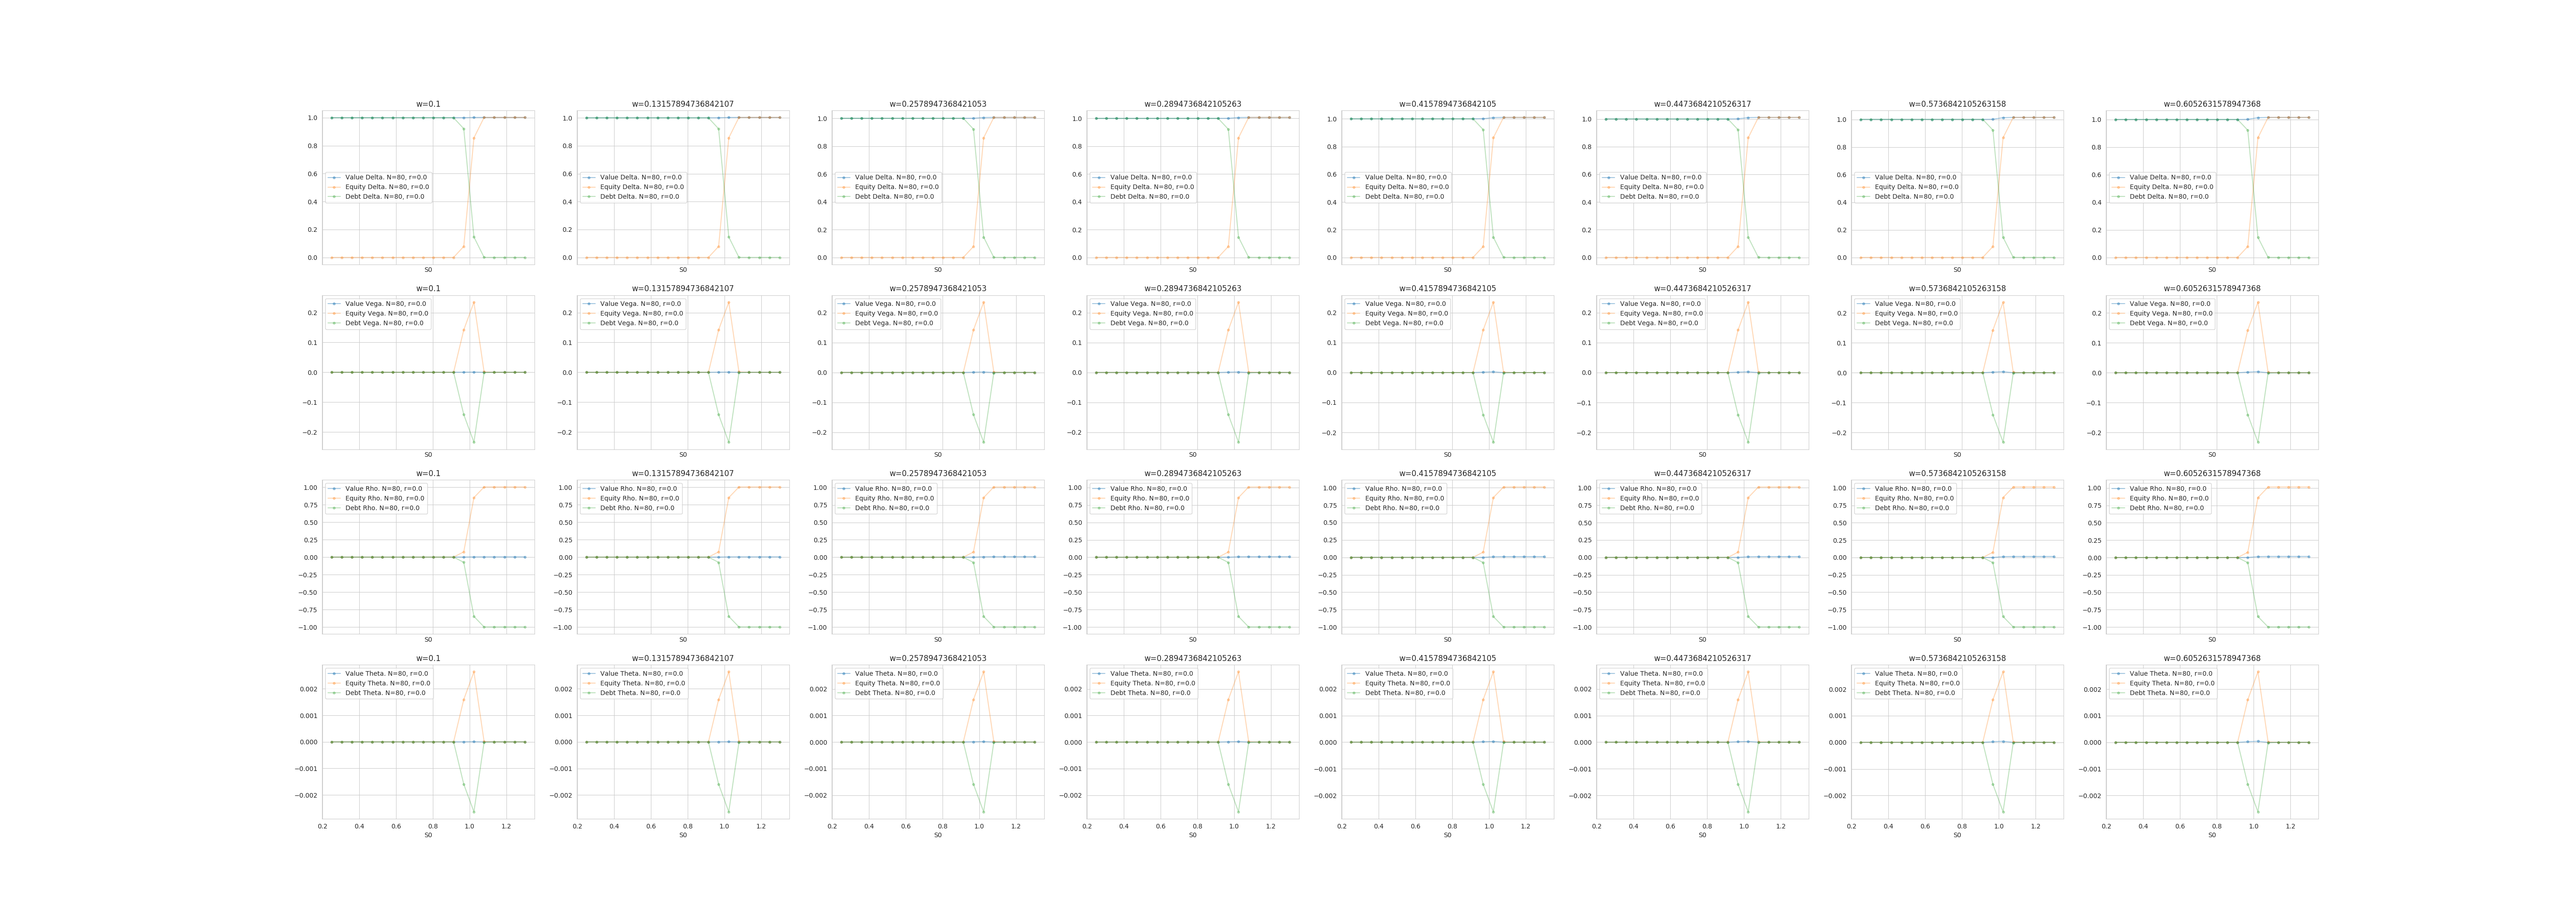
\includegraphics[trim={15cm 5cm 15cm 5cm},width=1.1\paperwidth]{greeks_1}
    %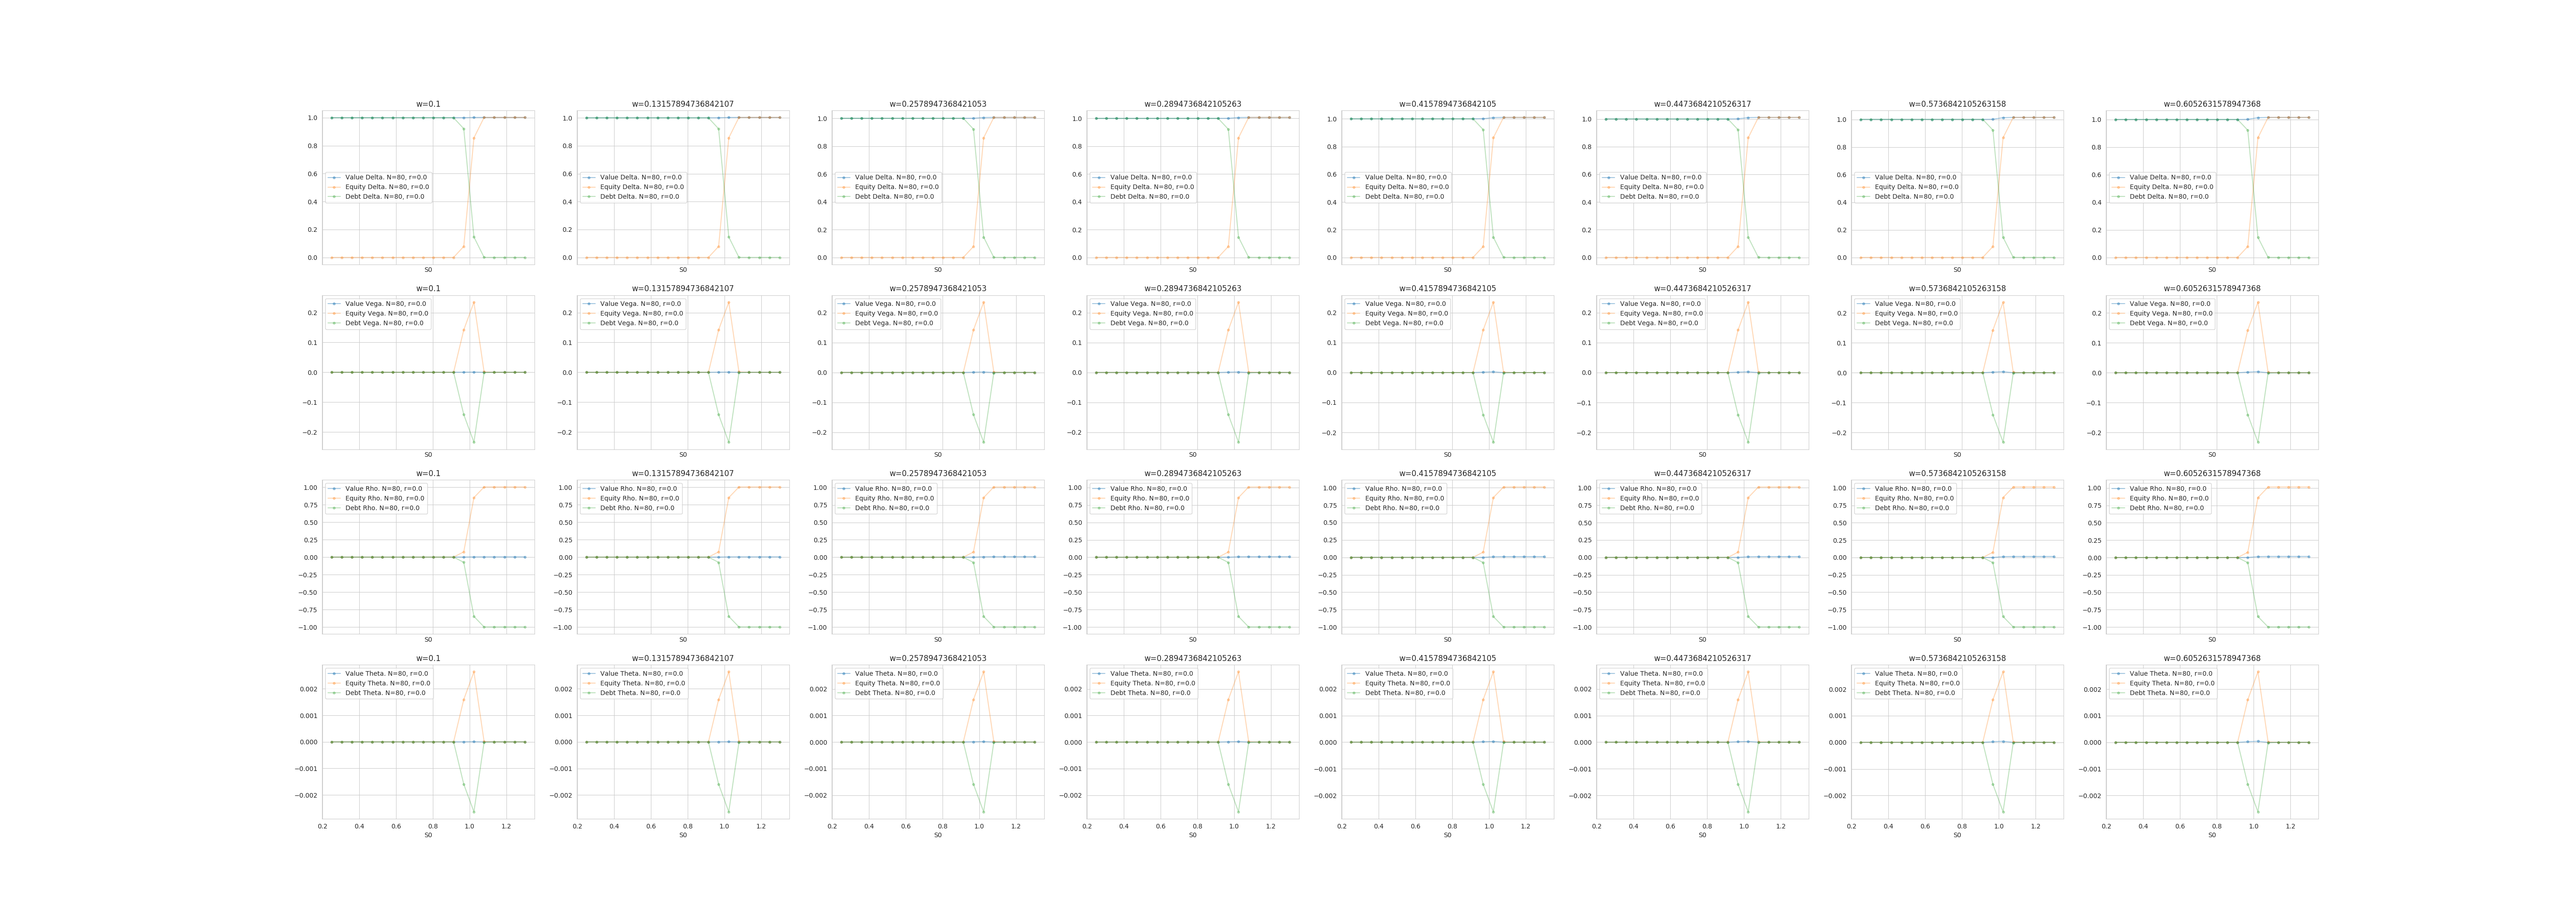
\includegraphics[angle=90,origin=c,width=0.8\linewidth,trim={15cm 5cm 15cm 5cm}]{greeks_1}
    \caption{Greeks as function of $S_0$}
    \label{fig:greeks_1}
\end{sidewaysfigure}

\missingfigure[figcolor=white]{Greeks as function of exogenous assets}
\end{document}
